\section{Vector Space Retrieval Model: Doc Length Normalization}


\subsection{Pivoted Length Normalization}

\textbf{Pivoted length normalizer}: use average doc length as <<pivot>>\footnote{Pivot - стержень; точка опоры, вращения}. Normalizer = 1 if $\abs{d}$ = average doc length (avdl).

\begin{figure}[H]
    \centering
    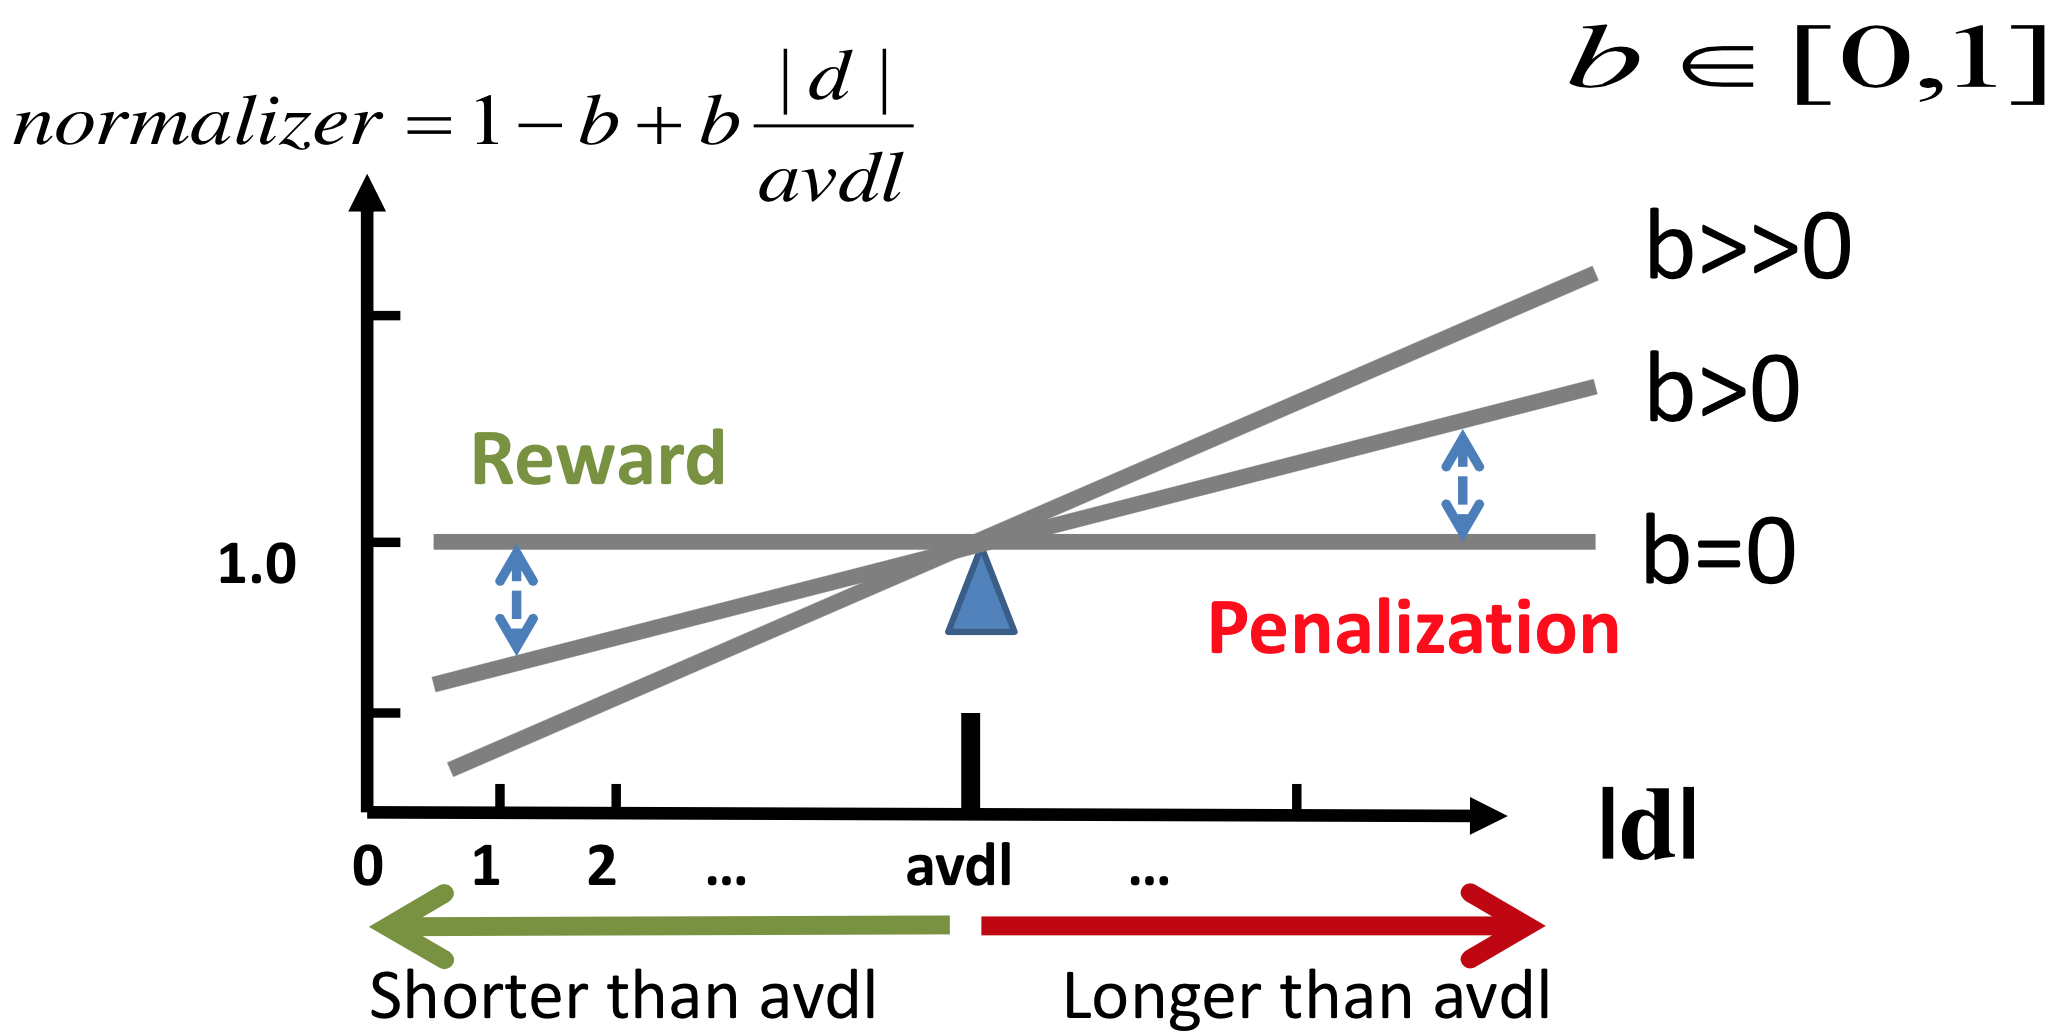
\includegraphics[width=0.75\linewidth]{pivoted_length_norm.png}
\end{figure}



\subsection{State of the Art VSM Ranking Functions}

Pivoted Length Normalization VSM [Singhal et al 96]:
\begin{equation*}
f(q, d) = \sum_{w \in q \cap d} c(w, q) \frac{\ln[1+\ln(1+c(w, d))]}{1-b+b\frac{|d|}{avdl}} \log \frac{M+1}{df(w)}
\end{equation*}


\href{https://ru.wikipedia.org/wiki/Okapi_BM25}{BM25/Okapi} [Robertson \& Walker 94]:
\begin{equation*}
f(q, d) = \sum_{w \in q \cap d} c(w, q) \frac{(k+1) c(w, d)}{c(w, d) + k\left(1-b+b\frac{|d|}{avdl}\right)} \log \frac{M+1}{df(w)}
\end{equation*}


\subsection{Further Improvement of VSM?}
\begin{itemize}
\item Improved instantiation of dimension?
\begin{itemize}
\item  stemmed words, stop word removal, phrases, latent semantic indexing (word clusters), character n-grams, ...
\item  bag-of-words with phrases is often sufficient in practice
\item  Language-specific and domain-specific tokenization is important to
ensure “normalization of terms”
\end{itemize}

\item  Improved instantiation of similarity function?
\begin{itemize}
\item  cosine of angle between two vectors?
\item  Euclidean?
\item  dot product seems still the best (sufficiently general especially with appropriate term weighting)
\end{itemize}
\end{itemize}


\subsection{Further Improvement of BM25}
\begin{itemize}
\item BM25F [Robertson \& Zaragoza 09]
\begin{itemize}
\item Use BM25 for documents with structures (<<F>>=fields)
\item Key idea: combine the frequency counts of terms in all fields and then apply BM25 (instead of the other way)
\end{itemize}

\item BM25+ [Lv \& Zhai 11]
\begin{itemize}
\item Address the problem of over penalization of long documents
by BM25 by adding a small constant to TF
\item Empirically and analytically shown to be better than BM25
\end{itemize}
\end{itemize}



\subsection{Summary of Vector Space Model}
\begin{itemize}
\item Relevance(q,d) = similarity(q,d)
\item Query and documents are represented as vectors
\item Heuristic\footnote{Heuristic - эвристический} design of ranking function

\item Major term weighting heuristics 
\begin{itemize}
\item TF weighting and transformation 
\item IDF weighting
\item Document length normalization
\end{itemize}

\item BM25 and Pivoted normalization seem to be most effective
\end{itemize}

\begin{figure}[H]
    \centering
    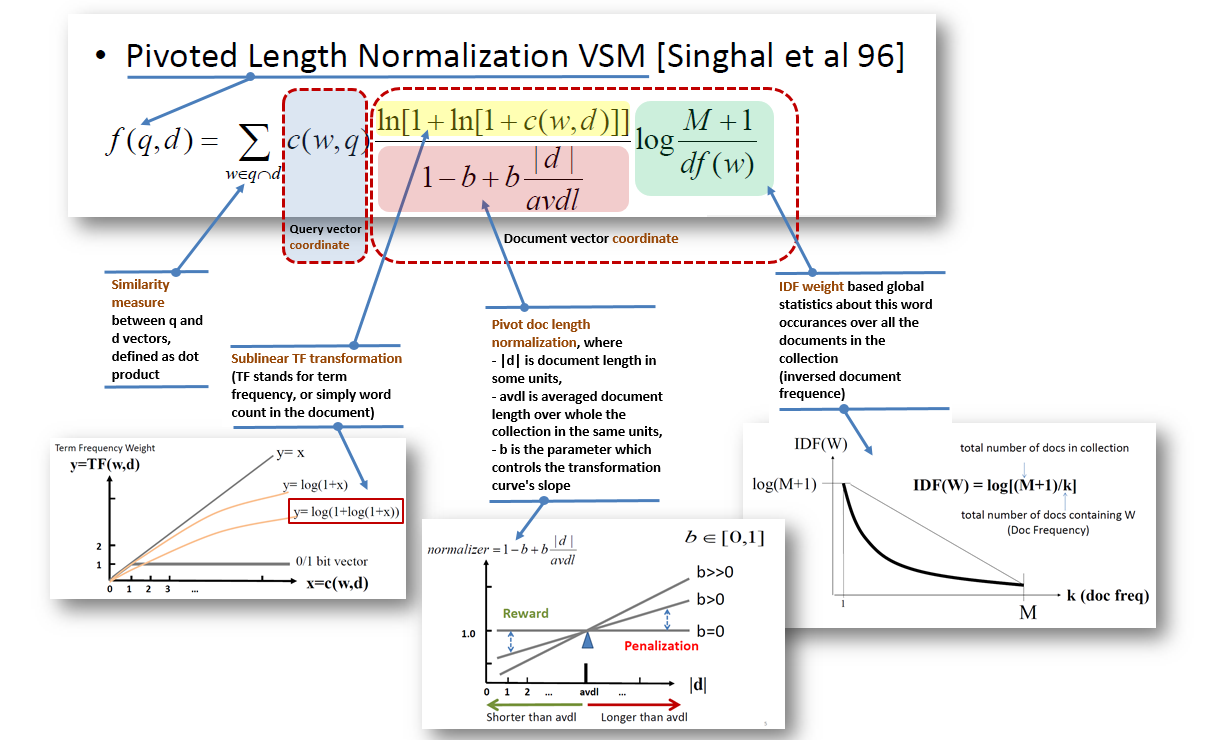
\includegraphics[width=\linewidth]{pivoted_length_normalization_vsm.png}
\end{figure}
\begin{figure}[H]
    \centering
    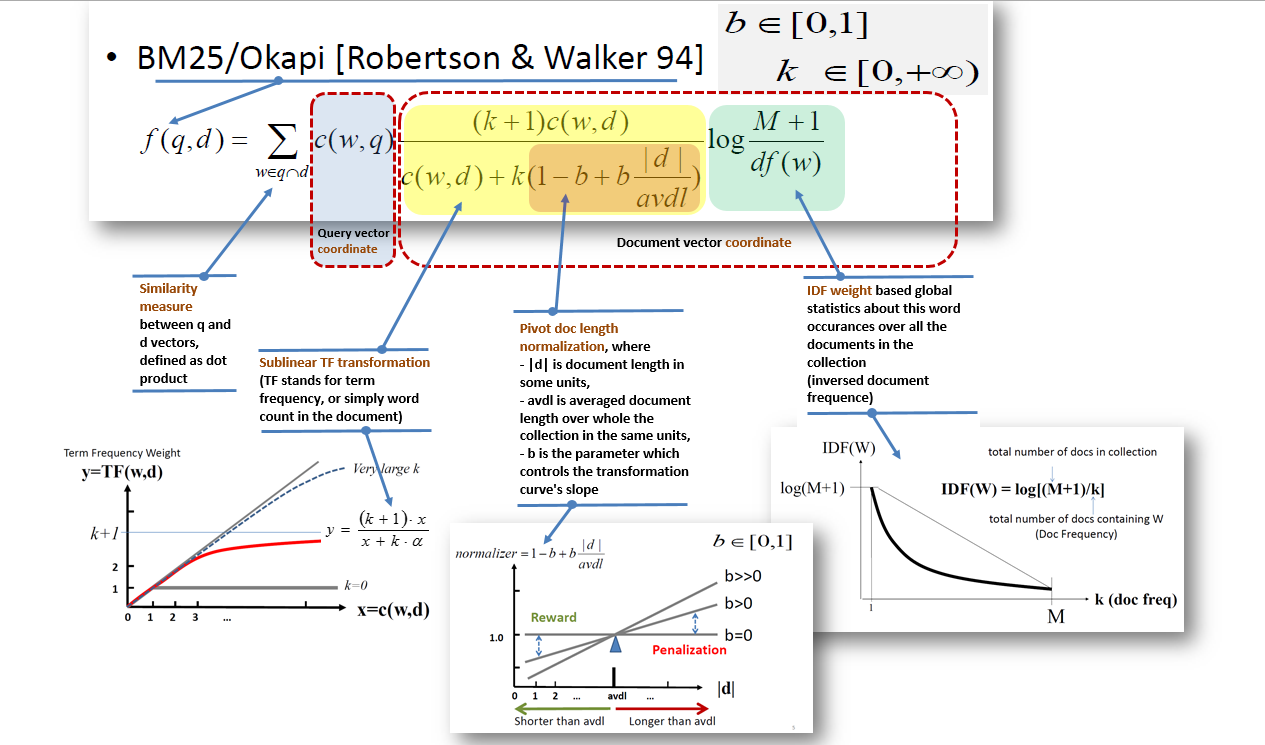
\includegraphics[width=\linewidth]{BM25_Okapi.png}
\end{figure}



\subsection{Recommended reading}
\begin{itemize}
\item A.Singhal, C.Buckley, and M.Mitra. <<Pivoted document length normalization>>. In Proceedings of ACM SIGIR 1996.
\item S. E. Robertson and S. Walker. <<Some simple effective approximations to the 2-Poisson model for probabilistic weighted retrieval>>, Proceedings of ACM SIGIR 1994.
\item S. Robertson and H. Zaragoza. <<The Probabilistic Relevance Framework: BM25 and Beyond>>, Found. Trends Inf. Retr. 3, 4 (April 2009).
\item Y. Lv, C. Zhai, <<Lower-bounding term frequency normalization>>. In Proceedings of ACM CIKM 2011.
\end{itemize}




